
\section{Erklärung zur Nutzung von KI-Werkzeugen}
%\addcontentsline{toc}{section}{Erklärung zur Nutzung von KI-Werkzeugen}

Bei der Erstellung dieses Exposés wurden KI-Werkzeuge unterstützend genutzt:

Verwendete Tools: Google Gemini 3.1 Pro

\begin{itemize}
    \item Hilfe bei der sprachlichen Überarbeitung und Verbesserung eigener Texte (Formulierungshilfe, Grammatik, und Rechtschreibprüfung)
    \item Hilfe bei LaTeX Befehlen und Formatierungen (z.B. Quellen in der references.bib oder Tabelle)
    \item Überprüfung auf Vollständigkeit der Anforderungen
    \item Unterstützung bei der Literaturrecherche
\end{itemize}

\section{Bewertungsmatrix (Excel)}
\label{sec:anhang_bewertungsmatrix}

In diesem Abschnitt ist die vollständige Bewertungsmatrix der Nutzwertanalyse abgebildet, die als Grundlage für die finale Auswertung diente. Aufgrund des Umfangs der Kriterien und Begründungen wurde die Darstellung der Excel-Datei in zwei Abbildungen aufgeteilt.

\begin{figure}[htbp]
    \centering
    % Passe den Dateinamen an deine Screenshots an
    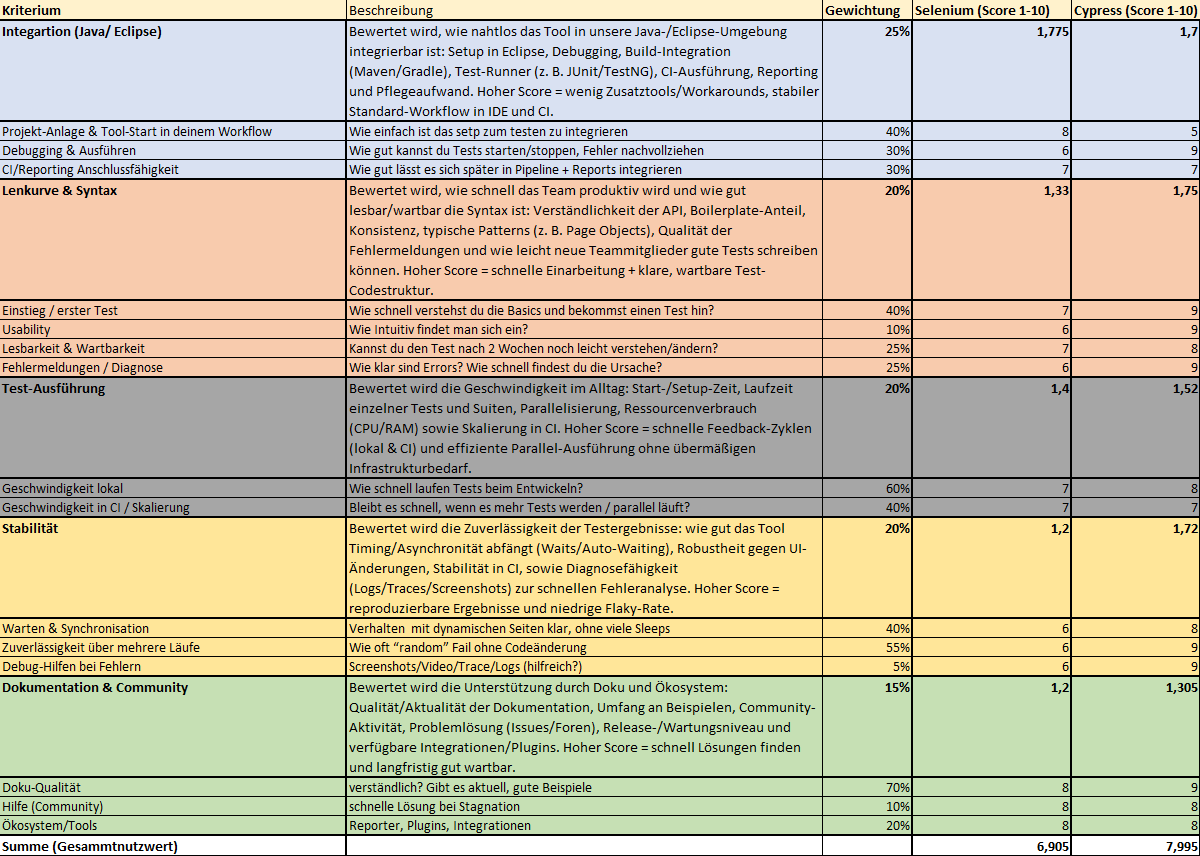
\includegraphics[width=\textwidth]{assets/img/BewertungsmatrixAusgefüllt.png}
    \caption{Bewertungsmatrix der Nutzwertanalyse (Selenium vs. Cypress) -- Teil 1}
    \label{fig:bewertungsmatrix_1}
\end{figure}

\begin{figure}[htbp]
    \centering
    % Passe den Dateinamen an deine Screenshots an
    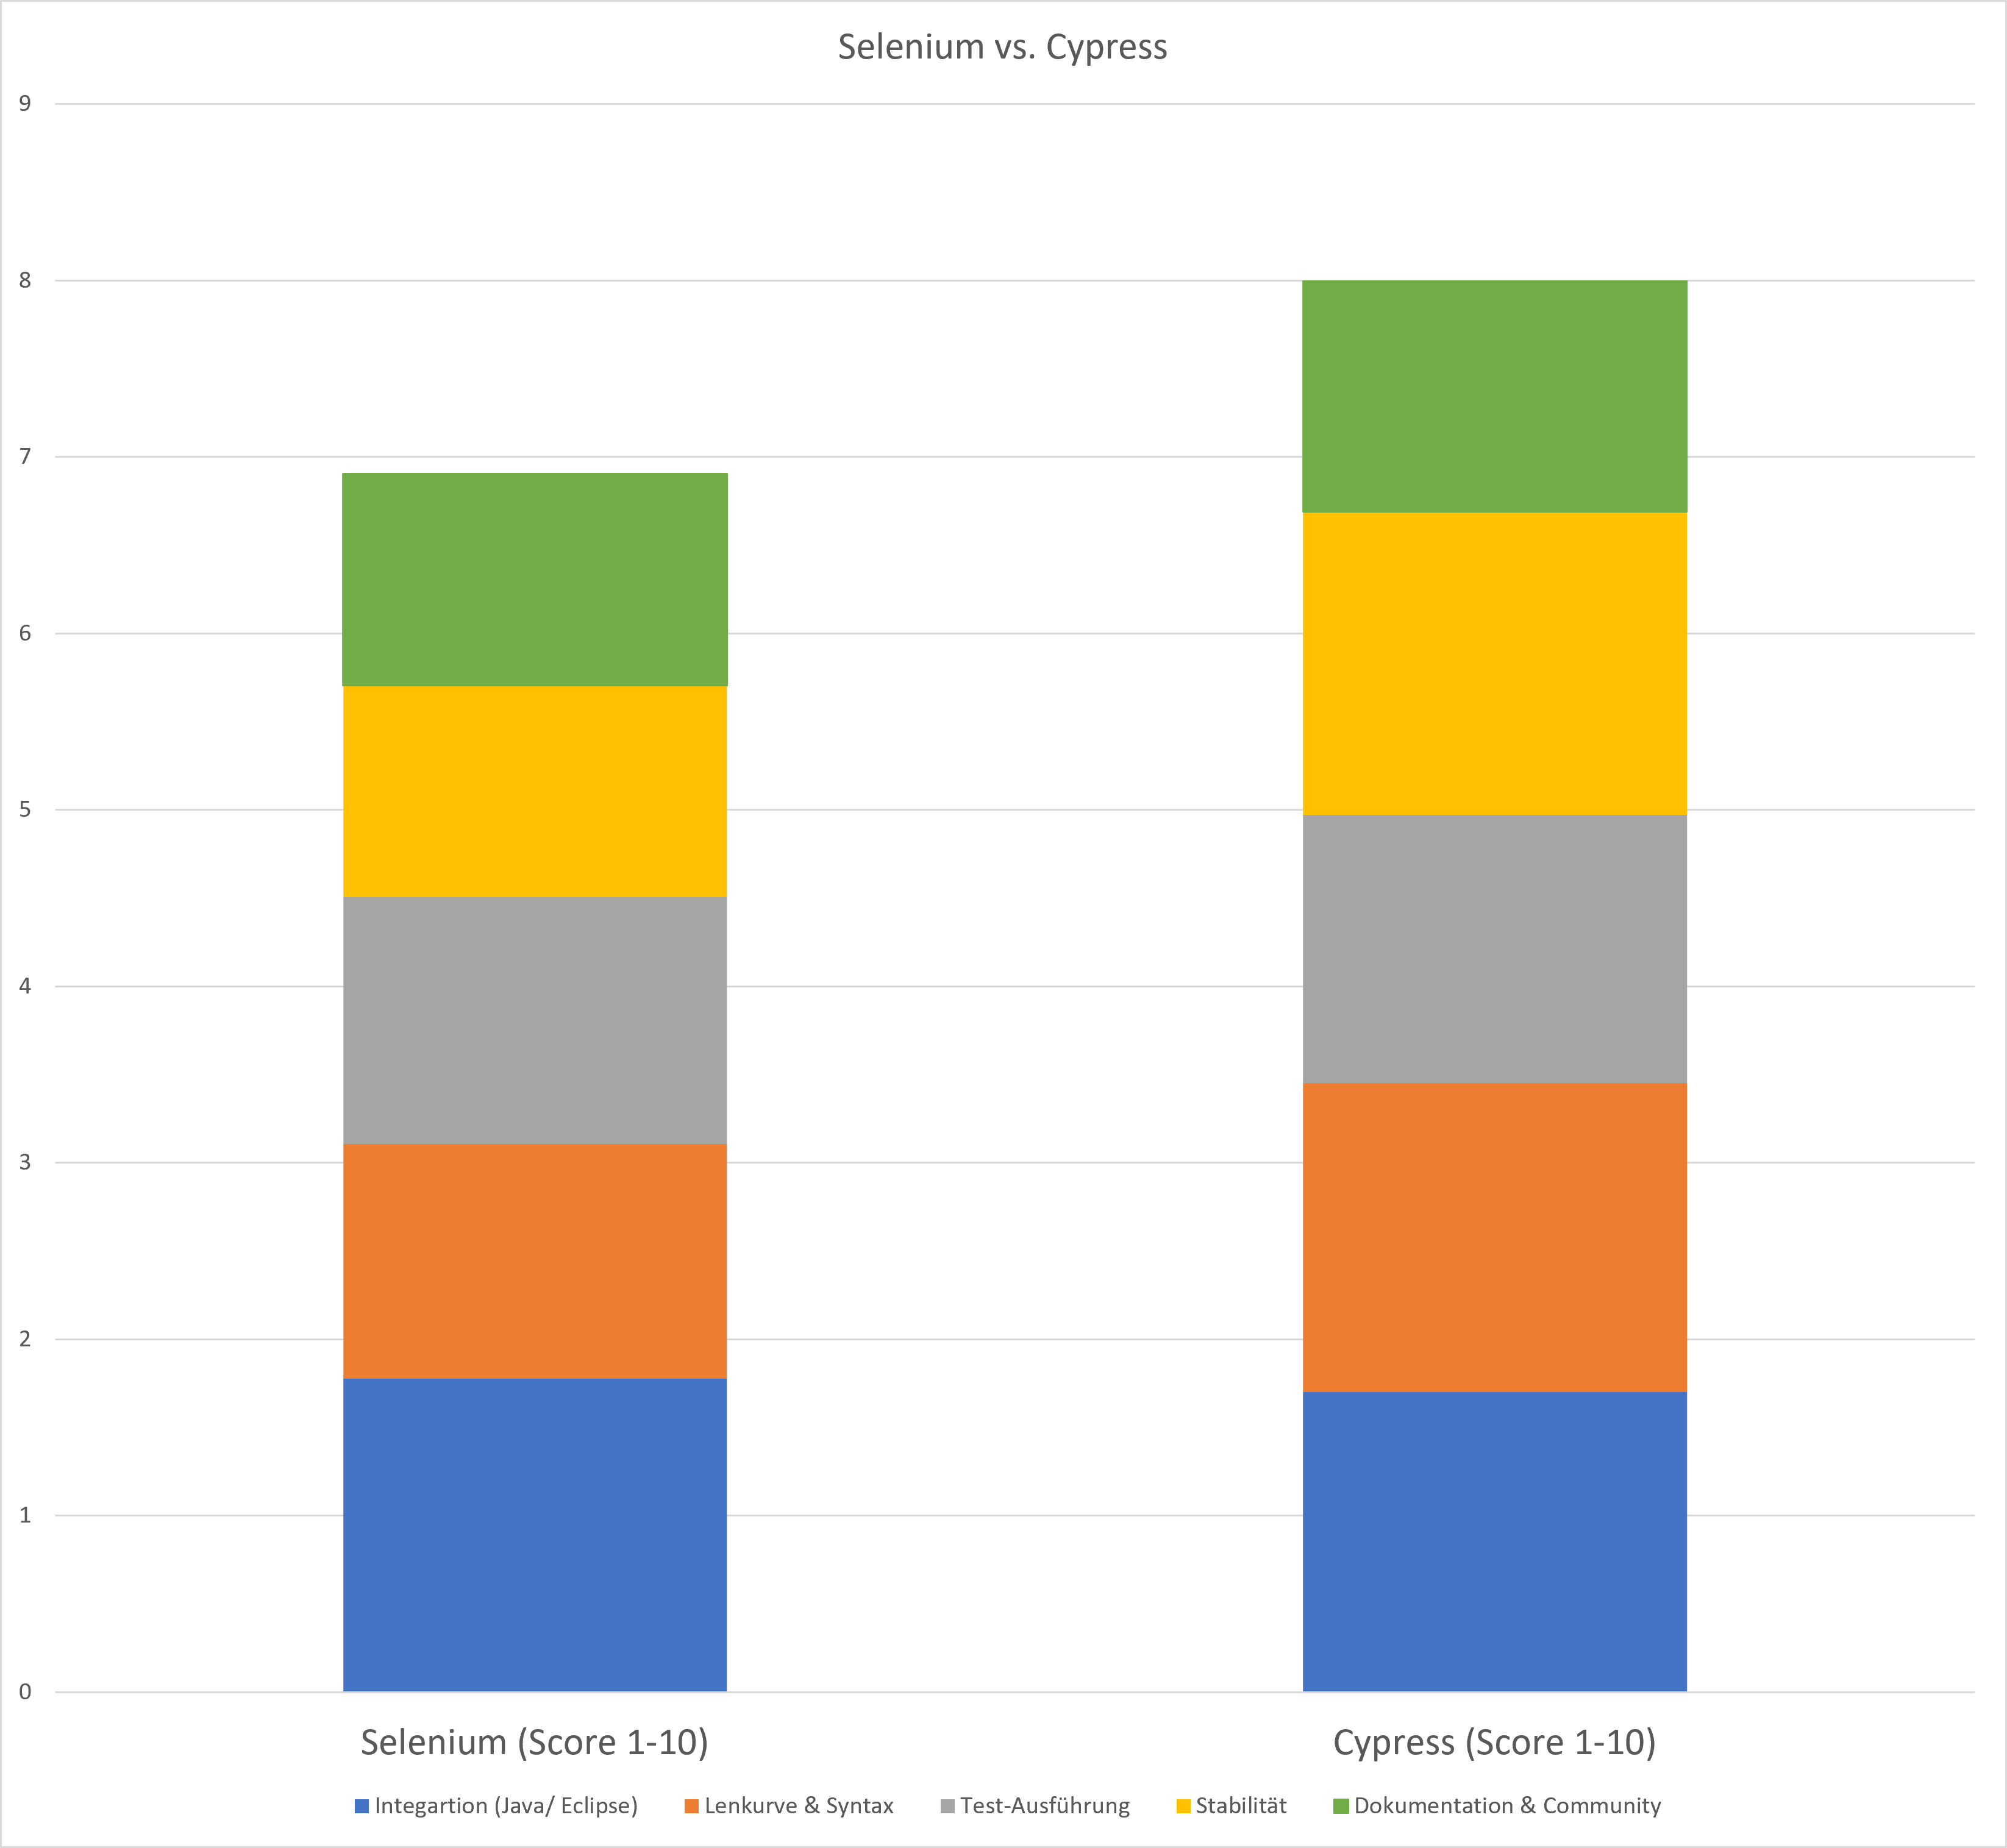
\includegraphics[width=\textwidth]{assets/img/DiagrammSelVsCy.png}
    \caption{Bewertungsmatrix der Nutzwertanalyse (Selenium vs. Cypress) -- Teil 2}
    \label{fig:bewertungsmatrix_2}
\end{figure}

\section{TestLog}
